\documentclass{article}
\linespread{1.3}
\usepackage[margin=50pt]{geometry}
\usepackage{amsmath, amsthm, amssymb, amsthm, tikz, fancyhdr, float, graphicx, spverbatim, systeme}
\pagestyle{fancy}
\renewcommand{\headrulewidth}{0pt}
\newcommand{\changefont}{\fontsize{15}{15}\selectfont}

\fancypagestyle{firstpageheader}{
  \fancyhead[R]{
    \changefont
    \parbox[t]{4cm}{ % Adjust width as needed
      Michael Huang\\
      EN.625.633.81\\
      Homework 8
    }
  }
}

\begin{document}

\thispagestyle{firstpageheader}
{\Large 

\section*{1.}

\subsection*{(a)} 

Assuming that \(X \sim N(0, \sigma^2)\), we aim to prove that \(E(\exp(-X^2)) = \frac{1}{\sqrt{2\sigma^2 + 1}}\):
\[
  E(\exp(-X^2)) = \int_{-\infty}^{\infty} e^{(-X^2)} \cdot f(x) dx
\]
By definition, we can substitute the pdf of the normal distribution (i.e. \(f(x) = \frac{1}{\sigma\sqrt{2\pi}} \cdot e^{-\frac{1}{2}(\frac{X - \mu}{\sigma})^2}\)):
\[
  = \int_{-\infty}^{\infty} e^{(-X^2)} \cdot \frac{1}{\sigma\sqrt{2\pi}} \cdot e^{-\frac{1}{2}(\frac{X - 0}{\sigma})^2}
\]
\[
  = \int_{-\infty}^{\infty} e^{-X^2} \cdot \frac{1}{\sigma\sqrt{2\pi}} \cdot e^{-\frac{X^2}{2\sigma^2}}
\]
\[
  = \frac{1}{\sigma\sqrt{2\pi}} \int_{-\infty}^{\infty} e^{-X^2} \cdot e^{-\frac{X^2}{2\sigma^2}}
\]
\[
  = \frac{1}{\sigma\sqrt{2\pi}} \int_{-\infty}^{\infty} e^{-X^2 - \frac{X^2}{2\sigma^2}}
\]
\[
  = \frac{1}{\sigma\sqrt{2\pi}} \int_{-\infty}^{\infty} e^{-X^2 (1 + \frac{1}{2\sigma^2})}
\]
\[
  = \frac{1}{\sigma\sqrt{2\pi}} \int_{-\infty}^{\infty} e^{-X^2 (\frac{2\sigma^2 + 1}{2\sigma^2})}
\]
This looks suspiciously close to the form of the pdf of the normal distribution which we just stated above, with the \(\frac{1}{\sigma^2}\) terms, and with this specific transformation: 
\[
  = \int_{-\infty}^{\infty} \frac{1}{\sigma\sqrt{2\pi}} \cdot e^{\frac{-X^2}{\frac{2\sigma^2}{2\sigma^2 + 1}}}
\]
So now we have a normal-ish distribution again. To simplify, we can try to remove the exponential by using the property that integral of the pdf of the normal distribution (or any valid pdf for that matter) = 1. Generally, for \(N(0, \sigma^2)\):
\[
  1 = \int_{-\infty}^{\infty} \frac{1}{\sigma\sqrt{2\pi}} \cdot e^{-\frac{1}{2}(\frac{x}{\sigma})^2}
\]
\[
  \sigma\sqrt{2\pi} = \int_{-\infty}^{\infty} e^{-\frac{1}{2}(\frac{x}{\sigma})^2}
\]
\[
  \sigma\sqrt{2\pi} = \int_{-\infty}^{\infty} e^{-\frac{x^2}{2\sigma^2}}
\]
\[
  \sqrt{2\pi\sigma^2} = \int_{-\infty}^{\infty} e^{-\frac{x^2}{2\sigma^2}}
\]
which we can extend to any SD = \(\sigma\) and variance = \(\sigma^2\). Using this, we can continue to solve:
\[
  = \int_{-\infty}^{\infty} \frac{1}{\sigma\sqrt{2\pi}} \cdot e^{\frac{-X^2}{\frac{2\sigma^2}{2\sigma^2 + 1}}}
\]
\[
  = \frac{1}{\sigma\sqrt{2\pi}} \sqrt{2\pi \cdot \frac{2\sigma^2}{2\sigma^2 + 1}} 
\]
\[
  = \frac{\sqrt{2\pi \cdot \frac{2\sigma^2}{2\sigma^2 + 1}} }{\sigma\sqrt{2\pi}}
\]
\[
  = \frac{\sqrt{2\pi \cdot \frac{2\sigma^2}{2\sigma^2 + 1}} }{\sqrt{2\pi\sigma^2}}
\]
\[
  = \sqrt{\frac{2\pi \cdot \frac{2\sigma^2}{2\sigma^2 + 1} }{2\pi\sigma^2}}
\]
\[
  = \sqrt{\frac{\frac{2\sigma^2}{2\sigma^2 + 1} }{\sigma^2}}
\]
\[
  = \sqrt{\frac{1}{2\sigma^2 + 1} }
\]
\[
  = \frac{1}{\sqrt{2\sigma^2 + 1}}
\]
exactly as we sought to find.

\subsection*{(b)}

\begin{spverbatim}
> basicMonteCarloInt_normal = function(n, sigma) {
+   
+   E_hat_vec = rep(0, (n-1));
+   upperConfBound_vec = rep(0, (n-1));
+   lowerConfBound_vec = rep(0, (n-1));
+   
+   actual_expectation = 1/sqrt(2*sigma^2 + 1);
+   
+   for (j in 1:(n-1)) {
+     normSample = rnorm((j+1), mean = 0, sd = sigma);
+     E_hat_vec[j] = mean(exp(-normSample^2));
+     estVar = mean((exp(-normSample^2) - E_hat_vec[j])^2)/j;
+     upperConfBound_vec[j] = E_hat_vec[j] + 1.96*sqrt(estVar);
+     lowerConfBound_vec[j] = E_hat_vec[j] - 1.96*sqrt(estVar);
+   }
+   
+   xValues = seq(1, (n-1), 1);
+   plot(xValues, E_hat_vec, type = "l",
+        main = paste("Monte Carlo Verification (sigma =", sigma, ")"));
+   lines(xValues, upperConfBound_vec, col = "red", lty = 4);
+   lines(xValues, lowerConfBound_vec, col = "red", lty = 4);
+   abline(h = actual_expectation, col = "blue", lwd = 2);
+   
+   
+ }
> 
> basicMonteCarloInt_normal(1000, 1)
> basicMonteCarloInt_normal(1000, 5)
> basicMonteCarloInt_normal(1000, 10)
\end{spverbatim}

\begin{figure}[H]
    \centering
    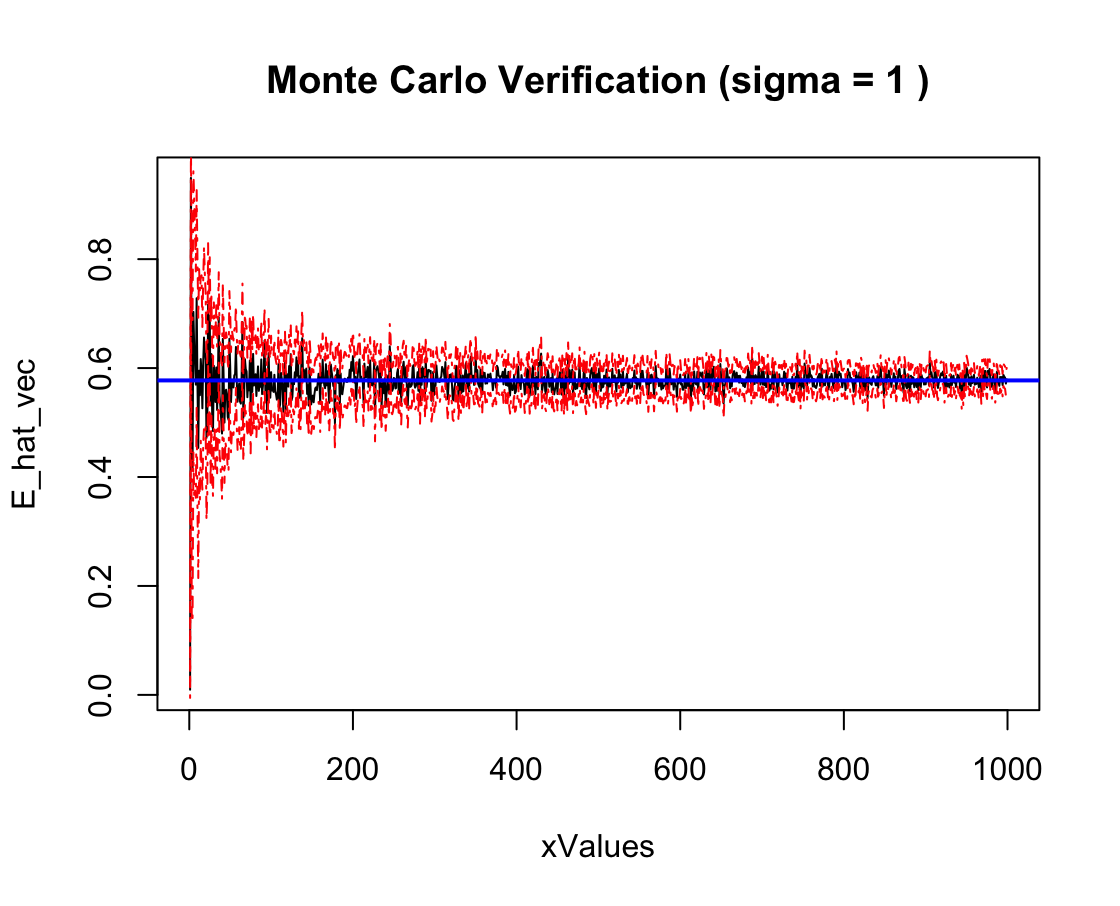
\includegraphics[width=0.75\textwidth]{1b_graph_sigma_1.png}
\end{figure}
\begin{figure}[H]
    \centering
    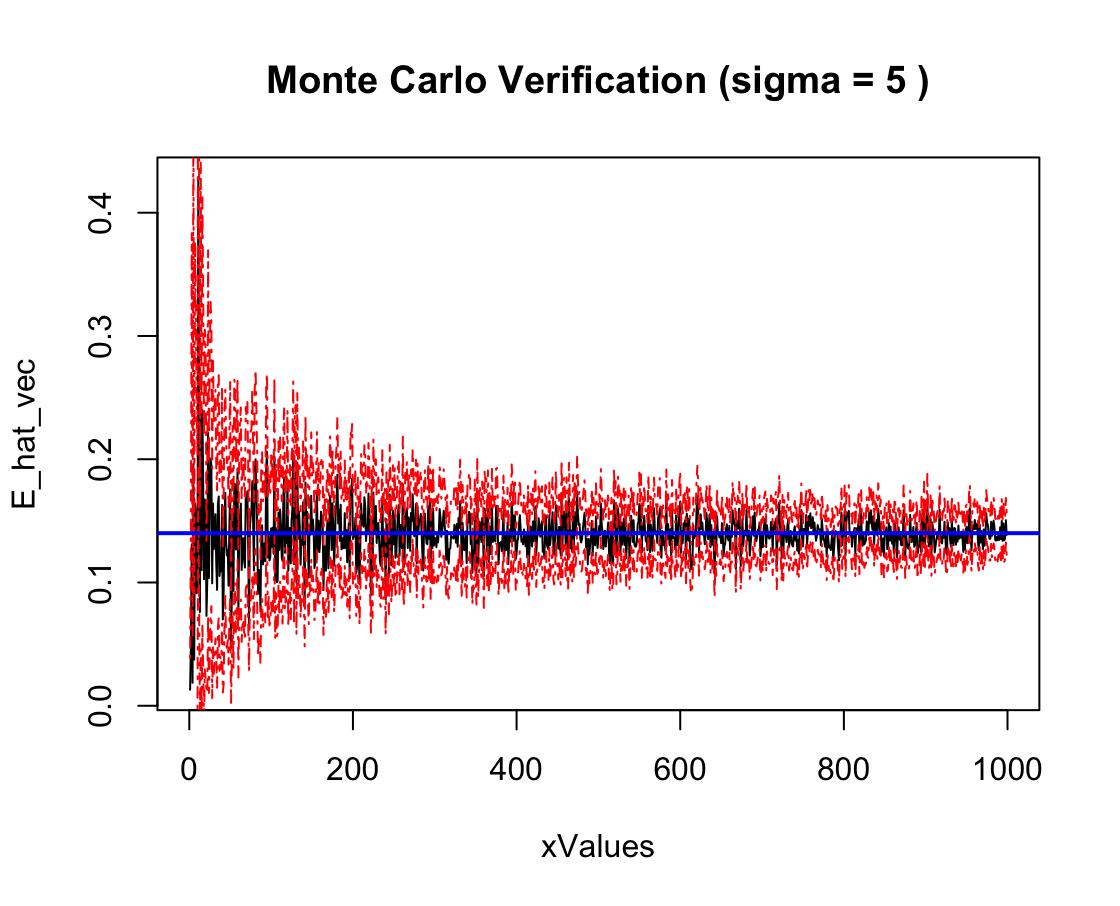
\includegraphics[width=0.75\textwidth]{1b_graph_sigma_5.png}
\end{figure}
\begin{figure}[H]
    \centering
    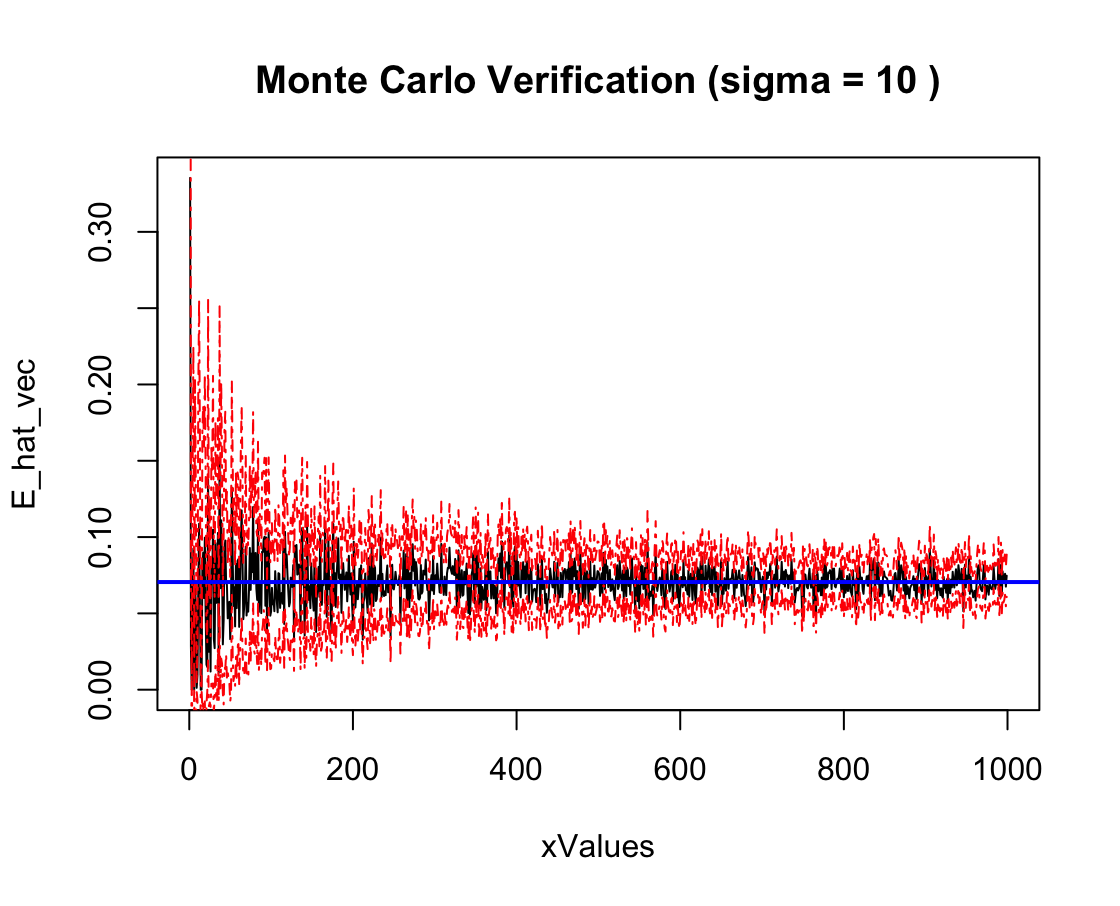
\includegraphics[width=0.75\textwidth]{1b_graph_sigma_10.png}
\end{figure}

The plots seem to show that this works pretty well, with the red values converging very closely to the blue actual/theoretical value.

}
{\Large 

\section*{2.}



}
{\Large 

\section*{3.}



}
{\Large 

\section*{4.}

\begin{figure}[H]
    \centering
    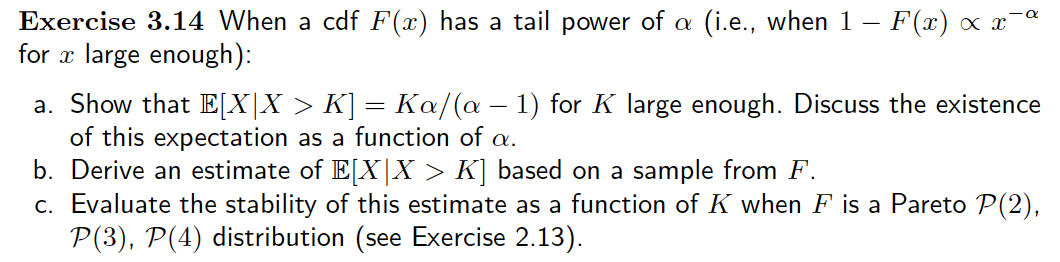
\includegraphics[width=1\textwidth]{Exercise3.14.png}
\end{figure}

\subsection*{(a)} 



\subsection*{(b)}



}

\end{document}